% ============================================================
% PHẦN SADGS — Slide bổ sung 1/8: Tổng quan cơ chế Structure-Aware Densification
% ============================================================

% --- Slide 1: Tổng quan cơ chế + bảng 6 hàm ---
\begin{frame}{SADGS (Lyu et al., SIGGRAPH 2026): Structure-Aware Densification}
\footnotesize
\begin{itemize}
    \item \textbf{SADGS} (\emph{Faster 3D Gaussian Splatting Convergence via Structure-Aware Densification}, MPI Informatik) kế thừa nền rasterizer/optimizer 3DGS nhưng \textbf{thay thế toàn bộ} cơ chế densify/prune bằng một cơ chế mới: so khớp \emph{screen-space extent} của mỗi Gaussian với \textbf{cấu trúc texture đa tỉ lệ} (multiscale image structure) của ảnh gốc.
    \item Ý tưởng cốt lõi: một Gaussian "đúng kích thước" khi trục chiếu của nó trên màn hình xấp xỉ \textbf{bước sóng cục bộ} (local wavelength) của texture mà nó phủ lên -- quá lớn $\Rightarrow$ alias/mờ chi tiết, quá nhỏ $\Rightarrow$ lãng phí.
\end{itemize}
\begin{table}
\centering
\begin{tabular}{ll}
\toprule
\textbf{Cơ chế} & \textbf{Hàm trong \texttt{gaussian\_model.py}} \\
\midrule
Đo tần số cấu trúc đa tỉ lệ & \texttt{utils/freq\_utils.py: update\_freq\_stats\_online} \\
Split dị hướng theo trục & \texttt{densify\_and\_split\_structgs} \\
Clone theo importance & \texttt{densify\_and\_clone\_structgs} \\
Giãn Gaussian dưới cỡ & \texttt{expand\_undersized\_gs} \\
Densify + prune 1 vòng & \texttt{densify\_and\_prune\_structgs} \\
Prune cuối (multi-view) & \texttt{final\_prune\_structgs} \\
\bottomrule
\end{tabular}
\end{table}
\begin{itemize}
    \item[$\Rightarrow$] 6 hàm này thay thế hoàn toàn cặp \texttt{densify\_and\_clone}/\texttt{densify\_and\_split} kiểu 3DGS gốc; không còn khái niệm "grad threshold cố định" duy nhất -- quyết định densify/prune giờ dựa trên \textbf{tỉ lệ nhất quán đa góc nhìn} (multiview-consistency ratio) của tín hiệu tần số.
    \item \alert{Lưu ý:} \texttt{expand\_undersized\_gs} và \texttt{final\_prune\_structgs} được định nghĩa đầy đủ trong code nhưng lời gọi của chúng trong \texttt{train.py} hiện \textbf{đang bị comment out} -- tức 2 cơ chế này \textbf{không} chạy mặc định trong luồng huấn luyện hiện tại (xem chi tiết ở các phần sau).
\end{itemize}
\centering
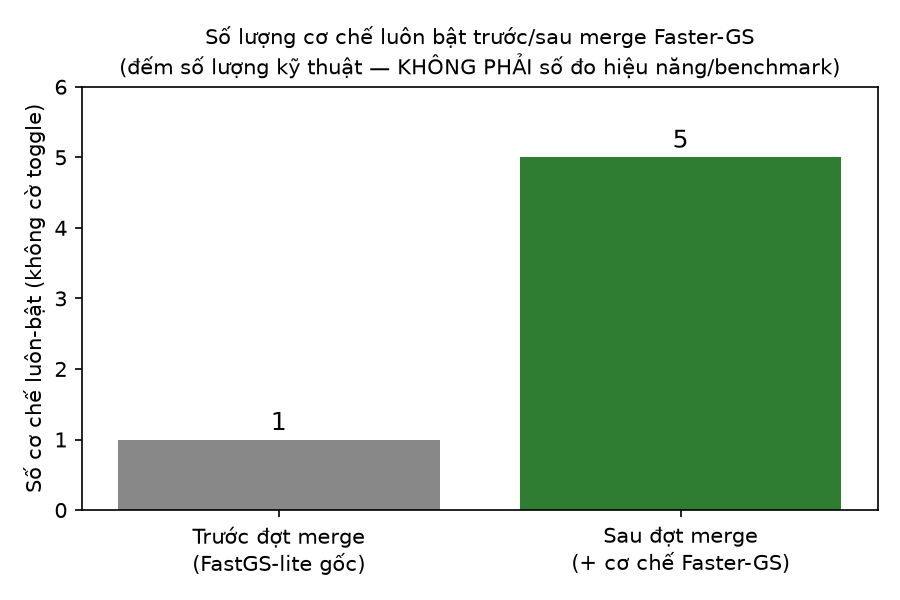
\includegraphics[width=0.3\linewidth]{../BOOK/fastergs_merge_figures/00_techniques_overview.png}
\captionof{figure}{\footnotesize Sơ đồ khối: đường đi dữ liệu từ structure tensor ảnh $\to$ eta 3 kênh $\to$ quyết định split/clone/prune}
\end{frame}

% --- Slide 2: Vì sao cần Structure-Aware? ---
\begin{frame}{Vì sao cần "Structure-Aware"? Trực giác Nyquist}
\begin{columns}[T]
\begin{column}{0.52\linewidth}
\footnotesize
\begin{itemize}
    \item \textbf{3DGS gốc}: tín hiệu densify duy nhất là \emph{screen-space positional gradient} trung bình -- Gaussian nào có gradient vị trí lớn (đóng góp nhiều vào việc giảm loss) thì được clone/split, bất kể kích thước hình học thực tế so với chi tiết ảnh. Rasterizer nền cũng giới hạn vùng ảnh hưởng bằng \emph{compact box} ($3\sigma$, hệ số \texttt{mult}$=0.7$) và một \emph{cost model} để tăng tốc, nhưng phần đó không đổi bản chất tín hiệu densify.
    \item \textbf{SADGS}: bỏ hẳn gradient làm tín hiệu chính, thay bằng \textbf{so khớp trực tiếp} kích thước Gaussian với tần số không gian thực đo được trên ảnh.
    \item Trực giác Nyquist: nếu trục Gaussian trên màn hình \textbf{lớn hơn} bước sóng cục bộ của texture $\Rightarrow$ dưới-lấy-mẫu (undersampling) $\Rightarrow$ mờ/alias chi tiết; nếu \textbf{nhỏ hơn nhiều} $\Rightarrow$ lãng phí bộ nhớ và compute mà không tăng chất lượng.
\end{itemize}
\end{column}
\begin{column}{0.46\linewidth}
\centering
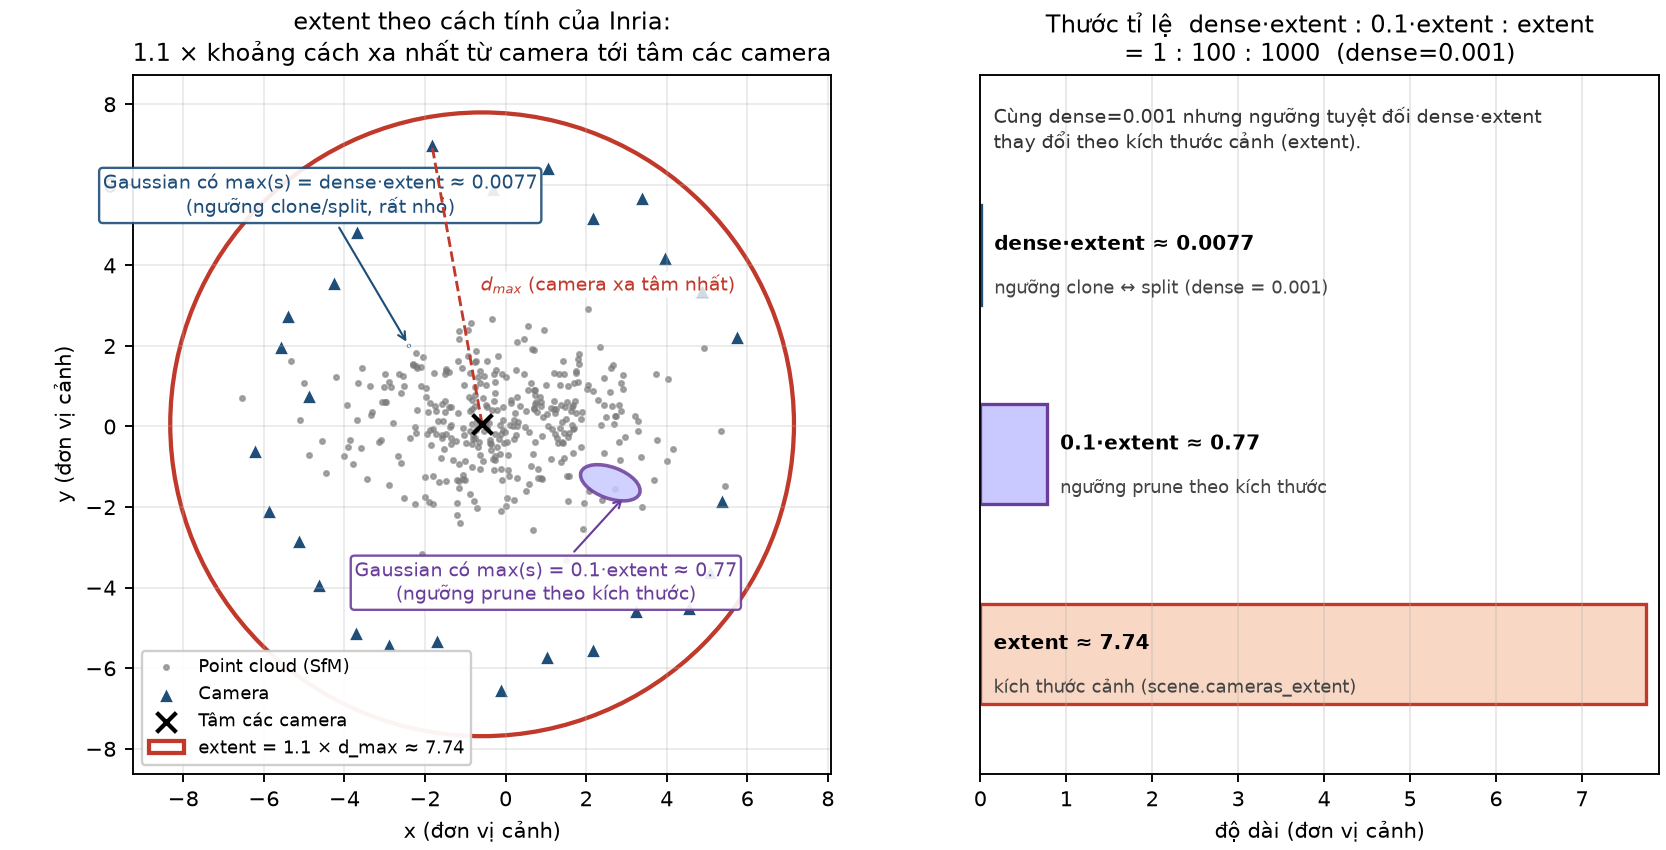
\includegraphics[width=\linewidth]{../BOOK/adc_3dgs/figures/fig_06_scene_extent.png}
\captionof{figure}{\footnotesize Phạm vi cảnh (scene extent) làm cơ sở chuẩn hoá ngưỡng kích thước Gaussian -- điểm khác biệt so với gradient thuần tuý của 3DGS gốc.}
\end{column}
\end{columns}
\end{frame}

% --- Slide 3: Dòng thời gian nghiên cứu + bảng so sánh 2 cột ---
\begin{frame}{Dòng thời gian: 3DGS $\to$ SADGS}
\footnotesize
\begin{itemize}
    \item \textbf{3DGS} (Kerbl et al., SIGGRAPH 2023): đặt nền móng densify/prune dựa trên gradient vị trí tích luỹ, split đẳng hướng bằng lấy mẫu ngẫu nhiên $\mathcal{N}(0, \mathrm{diag}(s^2))$.
    \item \textbf{SADGS} (Lyu et al., SIGGRAPH 2026 -- MPI Informatik, Cambridge, VIA): thay tín hiệu bằng tần số cấu trúc đa tỉ lệ $\eta$, split \textbf{dị hướng theo từng trục}, tích luỹ qua \textbf{nhiều view} trước khi quyết định.
\end{itemize}
\begin{table}
\centering
\begin{tabular}{lcc}
\toprule
\textbf{Tiêu chí} & \textbf{3DGS gốc} & \textbf{SADGS} \\
\midrule
Tín hiệu densify & grad vị trí & tần số $\eta$ đa tỉ lệ \\
Split dị hướng theo trục & không & có ($k_\text{axis}=\lceil\sqrt{\eta_\text{axis}}\rceil$) \\
Số view dùng để quyết định & 1 (tức thời) & nhiều (multiview-consistency) \\
Lưới con khi split & ngẫu nhiên $\mathcal{N}(0,\mathrm{diag}(s^2))$ & lưới tất định theo trục \\
\bottomrule
\end{tabular}
\end{table}
\begin{itemize}
    \item[$\Rightarrow$] Sự khác biệt cốt lõi: SADGS chuyển từ "Gaussian nào đang gây loss lớn" (gradient, tức thời) sang "Gaussian nào có kích thước sai so với tần số ảnh thật, nhất quán qua nhiều góc nhìn" (structure-aware, tích luỹ).
\end{itemize}
\end{frame}

% --- Slide 4: Giới thiệu khái niệm eta bằng ví dụ trực giác ---
\begin{frame}{Khái niệm $\eta$: tỉ số kích thước Gaussian / bước sóng texture}
\begin{columns}[T]
\begin{column}{0.5\linewidth}
\footnotesize
\begin{itemize}
    \item Định nghĩa trực giác: $\eta = \dfrac{\text{độ dài trục Gaussian chiếu màn hình}}{\text{bước sóng cục bộ của texture}}$.
    \item Ví dụ đơn giản: một Gaussian có trục chiếu dài 8 pixel, phủ lên vùng có vân texture lặp lại mỗi 4 pixel (bước sóng $=4$) $\Rightarrow \eta = 8/4 = 2$.
    \item $\eta \approx 1$: kích thước Gaussian \textbf{vừa khớp} bước sóng -- điểm cân bằng Nyquist, không cần densify/prune thêm.
    \item $\eta > 1$ (ví dụ trên, $\eta=2$): Gaussian \textbf{quá to} so với chi tiết $\Rightarrow$ cần \textbf{split} để giảm kích thước, tăng độ phân giải cục bộ.
    \item $\eta < 1$ (ví dụ: trục 2 pixel trên vùng bước sóng 4 pixel $\Rightarrow \eta=0.5$): Gaussian \textbf{quá nhỏ} $\Rightarrow$ ứng viên cho \texttt{expand\_undersized\_gs} (giãn) hoặc giữ nguyên nếu vùng đã đủ mượt.
    \item Ngưỡng cứng dùng trong phân loại: \texttt{TAU\_HIGH}$=1.0$ (trên $\eta$ này coi là "high", cần split), \texttt{TAU\_LOW}$=0.1$ (dưới ngưỡng này coi là "low"). Công thức đầy đủ (2 chế độ \texttt{wavelength}/\texttt{projection}) sẽ trình bày ở phần tiếp theo.
\end{itemize}
\end{column}
\begin{column}{0.48\linewidth}
\centering
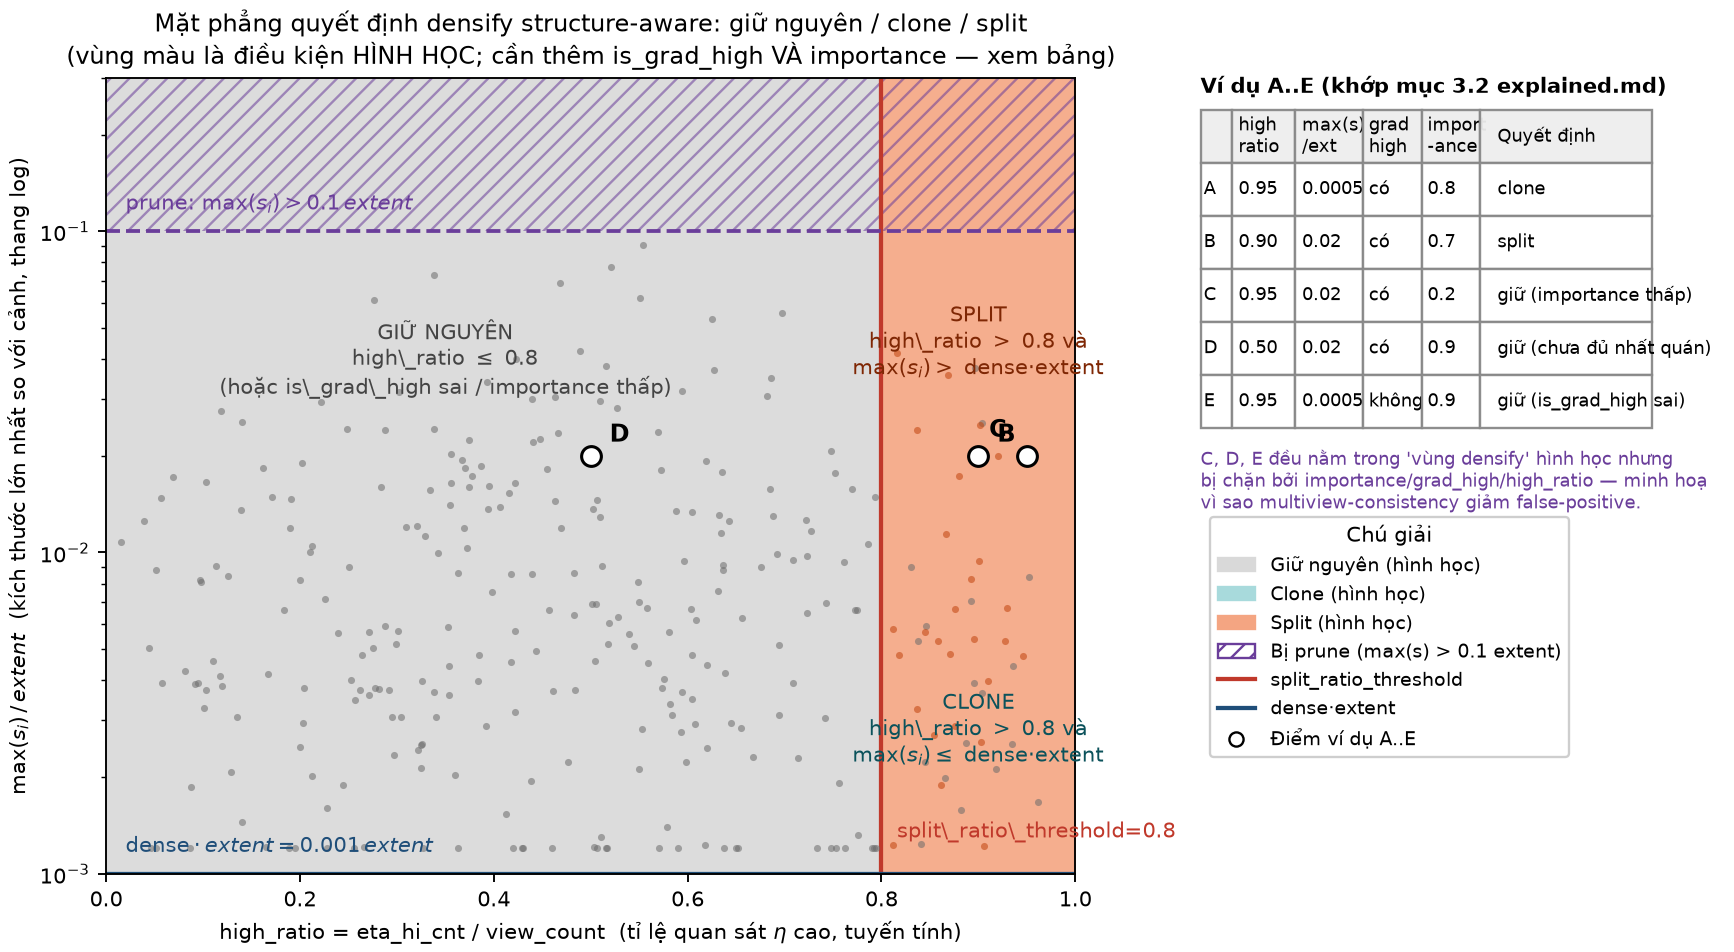
\includegraphics[width=\linewidth]{../BOOK/adc_3dgs/figures/fig_05_decision_plane.png}
\captionof{figure}{\footnotesize Mặt phẳng quyết định theo $\eta$: vùng split ($\eta$ cao), vùng ổn định ($\eta \approx 1$), vùng giãn/expand ($\eta$ thấp).}
\end{column}
\end{columns}
\end{frame}

% --- Slide 5: Lộ trình 8 phần tiếp theo ---
\begin{frame}{Lộ trình: 8 phần trình bày cơ chế SADGS}
\footnotesize
\begin{itemize}
    \item \textbf{Phần 2 -- Đo tần số}: \texttt{update\_freq\_stats\_online} tính structure tensor đa tỉ lệ, hai chế độ \texttt{eta\_compute\_mode} (\texttt{wavelength} dựa trị riêng $\lambda_1$, \texttt{projection} chiếu dạng toàn phương lên từng trục).
    \item \textbf{Phần 3 -- Clone}: \texttt{densify\_and\_clone\_structgs}, điều kiện dựa trên \texttt{importance\_score} (accum view count) so với ngưỡng $0.5$.
    \item \textbf{Phần 4 -- Split dị hướng}: \texttt{densify\_and\_split\_structgs}, lưới con tất định theo từng trục $k_\text{axis}=\lceil\sqrt{\eta_\text{axis}}\rceil$, khác 3DGS gốc lấy mẫu ngẫu nhiên.
    \item \textbf{Phần 5 -- Giãn Gaussian dưới cỡ}: \texttt{expand\_undersized\_gs}, bước giải tích $\Delta\log(\text{scale}) = -0.5\log(\eta)$ để đưa $\eta \to 1$ \alert{(hiện không được gọi trong \texttt{train.py})}.
    \item \textbf{Phần 6 -- Densify + prune 1 vòng}: \texttt{densify\_and\_prune\_structgs}, kết hợp \texttt{high\_ratio}/\texttt{split\_ratio\_threshold} $=0.8$ và \texttt{densify\_grad\_threshold}.
    \item \textbf{Phần 7 -- Prune cuối multi-view}: \texttt{final\_prune\_structgs}, loại bỏ khi \texttt{opacity}$<$\texttt{min\_opacity} hoặc \texttt{pruning\_score}$>0.9$ \alert{(hiện không được gọi trong \texttt{train.py})}.
    \item \textbf{Phần 8 -- Tổng kết}: so sánh hiệu quả, các tham số dead-code, và giới hạn thực nghiệm của SADGS so với 3DGS gốc.
\end{itemize}
\end{frame}
